\section{Proposed Scheme}

\begin{frame}{System Model \& Assumptions}
    \begin{columns}
        \begin{column}{0.55\textwidth}
            \textbf{Entities}
            \begin{itemize}
                \item \textbf{$D$} -- newly joined device (has a PUF, identity $ID_D$).
                \item \textbf{$AS$} -- authentication server: \emph{any} capable node pre-selected by the gateway (parent or non-parent).
                \item \textbf{$GW$} -- gateway / root node.
            \end{itemize}
            \vspace{0.25cm}
            \textbf{Assumptions}
            \begin{itemize}
                \item $GW$ shares a long-term key $K_{GW\text{-}AS}$ with each AS.
                \item $D$ knows the address and identity $ID_{AS}$ of its AS.
                \item Nodes can do hash, AES, XOR, AND, concat, and PUF eval.
            \end{itemize}
        \end{column}
        \begin{column}{0.45\textwidth}
            \begin{block}{Three protocol phases}
                \begin{enumerate}
                    \item \textbf{Enrolment} \\ {\footnotesize (once, secure channel)}
                    \item \textbf{Authentication} \\ {\footnotesize (open channel)}
                    \item \textbf{Key Exchange} \\ {\footnotesize (open channel)}
                \end{enumerate}
            \end{block}
            \begin{exampleblock}{Decoupling}
                \footnotesize Authentication is \emph{decoupled} from network joining --
                no parent is overwhelmed by its children.
            \end{exampleblock}
        \end{column}
    \end{columns}
\end{frame}

\begin{frame}{Network Topology -- Decoupled Authentication}
    \centering
    \scalebox{0.9}{%
    \begin{tikzpicture}[
        every node/.style={font=\footnotesize},
        relay/.style={circle, draw=black!55, fill=gray!12, minimum size=7mm, thick},
        gw/.style   ={circle, draw=iitblue, fill=iitblue!18, minimum size=11mm,
                      very thick, font=\footnotesize\bfseries},
        dev/.style  ={circle, draw=accentred, fill=accentred!15, minimum size=9mm,
                      very thick, font=\footnotesize\bfseries},
        as/.style   ={circle, draw=accentgreen, fill=accentgreen!18, minimum size=10mm,
                      very thick, font=\footnotesize\bfseries},
        link/.style ={draw=black!45, thick},
        auth/.style ={draw=accentgreen, very thick, dashed,
                      {Latex[length=2mm]}-{Latex[length=2mm]}},
    ]
        % Gateway / root
        \node[gw]    (gw) at (0,2.4)    {GW};
        % Level-1 relays
        \node[relay] (n1) at (-3,1.2)   {};
        \node[relay] (n2) at (3,1.2)    {};
        % Level-2 nodes
        \node[as]    (as) at (-4,0)     {AS};
        \node[relay] (n3) at (-1.8,0)   {};
        \node[relay] (n4) at (1.8,0)    {};
        \node[relay] (n5) at (4,0)      {};
        % Level-3 new device
        \node[dev]   (d)  at (1.8,-1.2) {D};

        % RPL routing tree (data path to GW)
        \draw[link] (gw) -- (n1);
        \draw[link] (gw) -- (n2);
        \draw[link] (n1) -- (as);
        \draw[link] (n1) -- (n3);
        \draw[link] (n2) -- (n4);
        \draw[link] (n2) -- (n5);
        \draw[link] (n4) -- (d);

        % Decoupled authentication + key exchange (D <-> AS, off the parent path)
        \draw[auth] (d) to[out=-90,in=-90,looseness=0.7]
              node[midway,below,text=accentgreen]{\scriptsize authentication} (as);
    \end{tikzpicture}}

    \vspace{0.2cm}
    {\footnotesize
    \textcolor{accentred}{\textbf{D}} new device \;\textbar\;
    \textcolor{accentgreen}{\textbf{AS}} gateway-selected authenticator \;\textbar\;
    \textcolor{iitblue}{\textbf{GW}} gateway / root}

    \vspace{0.1cm}
    {\footnotesize \textbf{Decoupling:} D's authenticator (AS) may or may not be its RPL parent --
    GW may pick any capable node, so no single parent is overloaded.}
\end{frame}

\begin{frame}{Key Idea 1 -- Per-Session Pseudonym Rotation}
    \begin{columns}
        \begin{column}{0.55\textwidth}
            \begin{itemize}
                \item Real $ID_D$ is sent \textbf{only once}, over the secure enrolment channel.
                \item Every open-channel message uses a pseudonym:
                $$\mathit{PID} = H(ID_D \,\|\, m_{\mathrm{curr}})$$
                \item After each key exchange, $m_{\mathrm{curr}} \!\rightarrow\! m_{\mathrm{new}}$,
                so $\mathit{PID}$ rotates.
                \item $H$ is one-way and $m_{\mathrm{curr}}$ is private $\Rightarrow$
                consecutive pseudonyms are \textbf{computationally unlinkable}.
            \end{itemize}
        \end{column}
        \begin{column}{0.45\textwidth}
            \begin{block}{Effect}
                \centering
                \footnotesize
                Session 1: $\mathit{PID}_1 = H(ID_D \| m_1)$ \\[0.2cm]
                Session 2: $\mathit{PID}_2 = H(ID_D \| m_2)$ \\[0.2cm]
                $\cdots$ \\[0.2cm]
                \textbf{An observer cannot link}
                $\mathit{PID}_1, \mathit{PID}_2, \ldots$ to the same device.
            \end{block}
        \end{column}
    \end{columns}
\end{frame}

\begin{frame}{Phase 1 -- Node Enrolment (Secure Channel)}
    \begin{columns}
        \begin{column}{0.46\textwidth}
            \footnotesize
            \begin{itemize}
                \item $D \to AS$: request + $ID_D$.
                \item $AS$ issues challenge $c_D$ and session random $m_D$.
                \item $D$ computes PUF response $R_D=\mathsf{PUF}_D(c_D)$, picks secret $y_D$,
                returns $(y_D, R_D, c_{AS\text{-}D})$.
                \item $AS$ folds $H(y_D)$ into accumulator $T_{\mathsf{Acc}}$ (bitwise AND),
                stores $\Phi_{AS\text{-}D}=R_{AS\text{-}D}\oplus R_D$.
                \item \textbf{Pseudonym init:} $AS$ sets $\mathit{PID}_{\mathrm{curr}}=H(ID_D\|m_{\mathrm{curr}})$,
                $\mathit{PID}_{\mathrm{old}}=\varepsilon$ -- the initial \textbf{dual state}.
            \end{itemize}
        \end{column}
        \begin{column}{0.54\textwidth}
            \centering
            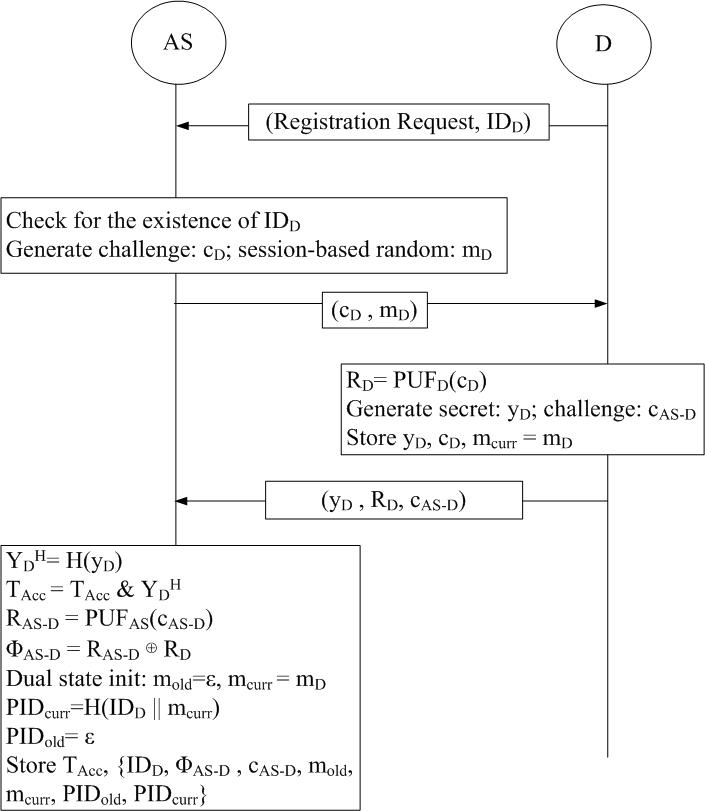
\includegraphics[width=\textwidth]{fig_enrollment.jpg}
        \end{column}
    \end{columns}
\end{frame}

\begin{frame}{Phase 2 -- Node Authentication (Open Channel)}
    \begin{columns}
        \begin{column}{0.46\textwidth}
            \footnotesize
            \begin{itemize}
                \item $D$ regenerates $R_D$ from $c_D$ and computes $\mathit{PID}=H(ID_D\|m_{\mathrm{curr}})$.
                \item Sends masked tag
                $Y_{AS\text{-}D}^H = H(y_D)\oplus H(R_D\|m_{\mathrm{curr}}\|\mathit{PID}\|ts_1)$.
                \item Message: $(\mathit{PID},\, Y_{AS\text{-}D}^H,\, ts_1)$ -- \textbf{no $ID_D$}.
                \item $AS$ does a \textbf{dual-state lookup} ($\mathit{PID}_{\mathrm{curr}}$ or $\mathit{PID}_{\mathrm{old}}$),
                checks $ts_1$ freshness.
                \item $AS$ recovers $R_D'$, unmasks $Y_D^{H'}$, verifies via the
                \textbf{accumulator AND-check} ($T_{\mathsf{Acc}}^{\mathsf{new}}\!=\!T_{\mathsf{Acc}}$).
            \end{itemize}
        \end{column}
        \begin{column}{0.54\textwidth}
            \centering
            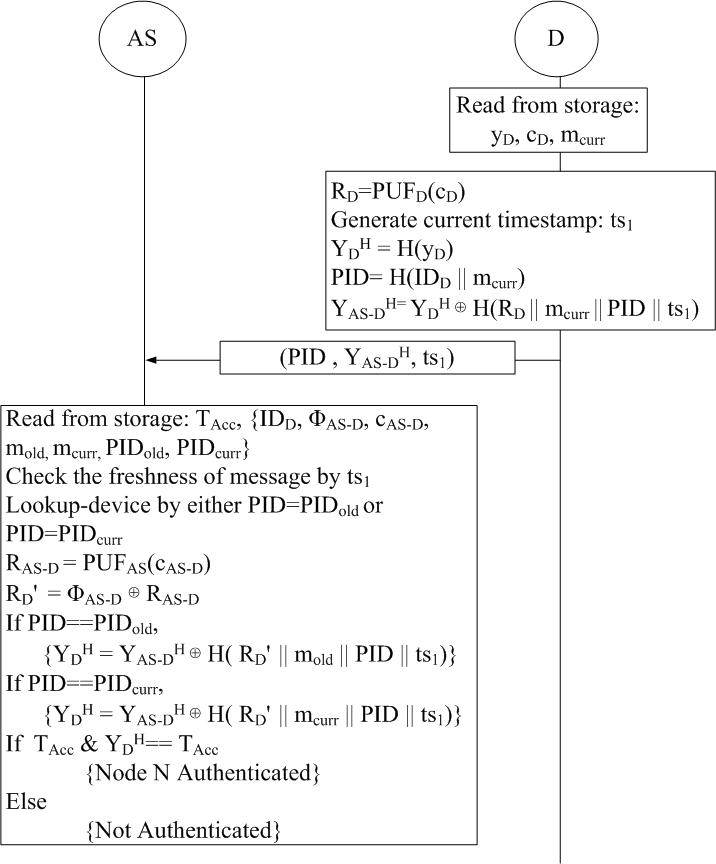
\includegraphics[width=\textwidth]{fig_auth.jpg}
        \end{column}
    \end{columns}
\end{frame}

\begin{frame}{Phase 3 -- Session Key Exchange (Open Channel)}
    \begin{columns}
        \begin{column}{0.46\textwidth}
            \footnotesize
            \begin{itemize}
                \item $AS$ draws fresh $n_1$, sets $m_{\mathrm{new}}=H(n_1)$.
                \item Session key $K_{GW\text{-}D}=H(R_D'\|m_{\mathrm{new}})$.
                \item New pseudonym $\mathit{PID}_{\mathrm{new}}=H(ID_D\|m_{\mathrm{new}})$.
                \item $AS \to GW$: $\mathsf{auth\_token}_D$ (encrypted under $K_{GW\text{-}AS}$, carries $K_{GW\text{-}D}$ + $\mathit{PID}_{\mathrm{new}}$).
                \item $AS \to D$: masked $m_H = m_{\mathrm{new}}\oplus H(\cdots)$ + $ts_2$.
                \item $D$ recovers $m_{\mathrm{new}}$, derives the \textbf{same} $K_{GW\text{-}D}$, rotates $\mathit{PID}$.
                \item $AS$ \& $GW$ advance state: old $\leftarrow$ curr, curr $\leftarrow$ new.
            \end{itemize}
        \end{column}
        \begin{column}{0.54\textwidth}
            \centering
            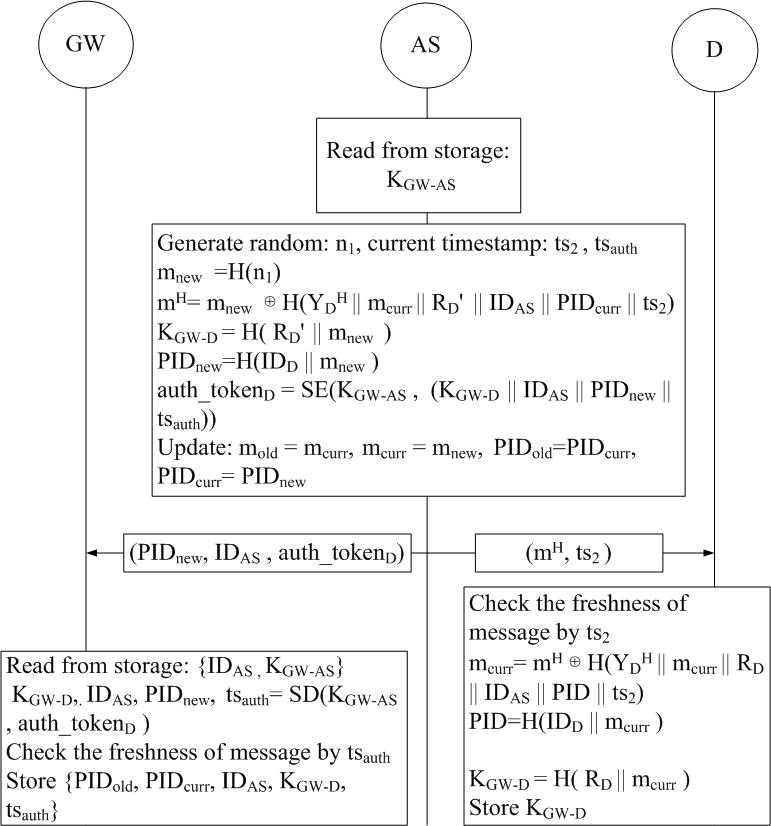
\includegraphics[width=\textwidth]{fig_keyex.jpg}
        \end{column}
    \end{columns}
\end{frame}

\begin{frame}{Key Idea 2 -- Dual-State Desynchronisation Recovery}
    \begin{columns}
        \begin{column}{0.5\textwidth}
            \textbf{The problem}
            \begin{itemize}
                \item In Phase 3, $AS$ sends $(m_H, ts_2)$ to $D$.
                \item If this packet is \textbf{lost}, $AS$ has already advanced to $m_{\mathrm{new}}$,
                but $D$ keeps stale $m_{\mathrm{curr}}$.
                \item $D$'s next $\mathit{PID}$ matches nothing $\Rightarrow$ authentication fails.
            \end{itemize}
            \vspace{0.2cm}
            \textbf{Base scheme (DAuth):} single state $\Rightarrow$ \textbf{full re-enrolment}.
        \end{column}
        \begin{column}{0.5\textwidth}
            \begin{block}{Our fix: dual state}
                $AS$ \& $GW$ keep \emph{both}
                $(m_{\mathrm{curr}},\mathit{PID}_{\mathrm{curr}})$ and
                $(m_{\mathrm{old}},\mathit{PID}_{\mathrm{old}})$.
            \end{block}
            \begin{itemize}\footnotesize
                \item Stale $D$ arrives with $\mathit{PID}=\mathit{PID}_{\mathrm{old}}$.
                \item $AS$ recognises it via dual-state lookup, verifies using $m_{\mathrm{old}}$,
                and re-synchronises -- \textbf{no re-enrolment}.
                \item $D$'s behaviour is \emph{identical}; only $AS$ adapts.
            \end{itemize}
            \begin{alertblock}{Trade-off}
                \footnotesize Tolerates a single consecutive loss; two slots balance storage vs.\ recovery depth.
            \end{alertblock}
        \end{column}
    \end{columns}
\end{frame}

\begin{frame}{Dual-State Recovery -- Algorithm}
    \begin{center}
        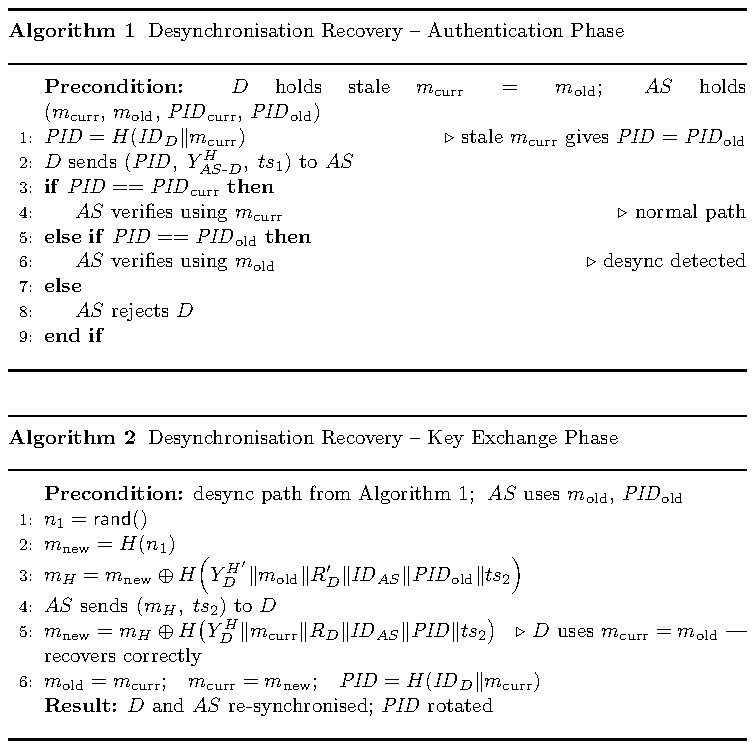
\includegraphics[width=0.62\textwidth,height=0.82\textheight,keepaspectratio]{fig_desync_algo.pdf}
    \end{center}
\end{frame}
